\chapter{Introduzione}

\section{Intelligenza Artificiale: una doppia sfida}

L'Intelligenza Artificiale si occupa della
\begin{enumerate}
	\item comprensione
	\item riproduzione
\end{enumerate}
del comportamento \textit{intelligente}.
\subsubsection{L'IA come scienza empirica}

L'approccio della psicologia cognitiva:\\
\textbf{\textit{Obiettivo}}:\ comprensione dell'intelligenza umana.\\
\textbf{\textit{Metodo}}:\ costruzione di modelli computazionali, verifica sperimentale.\\
\textbf{\textit{Criterio di successo}}:\ risolvere i problemi con gli stessi processi usati dall'uomo.

\subsubsection{L'IA come disciplina informatica}
L'approccio ``costruttivo'':\\
\textbf{\textit{Obiettivo}}:\ costruzione di entità dotate di razionalità.\\
\textbf{\textit{Metodo}}:\ codifica del pensiero razionale; comportamento razionale.\\
\textbf{\textit{Criterio di successo}}:\ l'importante è risolvere i problemi che richiedono intelligenza.

\subsection{Definizioni di IA}
\begin{table}[H]
	\centering
	\begin{tabular}{|l|p{13.5em}|p{13em}|}
		\hline
		        & Umanamente                                                                                                                                                                      & Razionalmente                                                                                                                                                                                                                                  \\\hline
		Pensare & ``\textit{L'automazione delle attività che associamo al pensiero umano, come il processo decisionale, la risoluzione di problemi, l'apprendimento}\dots''\newline[Bellman 1978] & ``\textit{Lo studio delle facoltà mentali attraverso l'uso di modelli computazionali}''\newline[Charniak, McDermott, 1985]                                                                                                                     \\\hline
		Agire   & ``\textit{L'arte di creare macchine che svolgono funzioni che richiedono intelligenza quando svolte da esseri umani}''\newline[Kurzweil 1990]                                   & ``\textit{Il ramo della scienza dei calcolatori che si occupa dell'automazione del comportamento intelligente}''\newline [Luger-Stubblefield 1993] \newline ``\textit{L'impresa di costruire artifatti intelligenti}''\newline [Ginsberg 1993] \\\hline
	\end{tabular}
\end{table}
\subsubsection{Da ``\textit{Strategic directions in Artificial Intelligence}''}

Il settore dell'IA consiste nell'indagine tecnologica e intellettuale, a lungo termine, che mira al raggiungimento dei seguenti obiettivi scientifici e pratici:
\begin{itemize}
	\item costruzione di macchine intelligenti, sia che operino come l'uomo che diversamente;
	\item formalizzazione della conoscenza e meccanizzazione del ragionamento, in tutti i settori di azione dell'uomo;
	\item comprensione mediante modelli computazionali della psicologia e comportamento di uomini, animali e agenti artificiali;
	\item rendere il lavoro con il calcolatore altrettanto facile e utile che del lavoro con persone, capaci, cooperative e possibilmente esperte.
\end{itemize}
Prendiamo per buona questa definizione:
\begin{center}
	\textit{L'arte di creare macchine che svolgono funzioni che richiedono intelligenza quando svolte da esseri umani}

	- Kurzweil, 1990
\end{center}
Ma cosa significa ``intelligente''?\ Settanta definizioni di intelligenza, di cui 35 fuori dal settore AI.\
È una qualità intrinseca o un comportamento?\
Difficile arrivare ad una definizione condivisa e completa perché esistono diversi tipi di ``intelligenza''.

Che tipo di capacità?
\begin{itemize}
	\item Capacità di simulare il comportamento umano?
	\item Capacità di ragionamento logico/matematico?
	\item Intelligenza come competenza ``da esperto''?
	\item Intelligenza come ``buon senso'' (common sense)?
	\item Capacità di interagire efficacemente con un ambiente?
	\item Capacità sociali, di comunicazione e coordinamento?
	\item Capacità di comprendere e provare emozioni? (intelligenza emozionale)
	\item Capacità di ``immagazzinare'' esperienza? Apprendere?
	\item Creatività?
\end{itemize}
Capacità di imitazione dell'uomo?\
\textbf{Il test di Turing} (1950):\ un tentativo di definizione operativa di intelligenza.\
Le previsioni di Turing:

\vspace{12pt}
\noindent``\textit{Credo che tra circa 50 anni sarà possibile programmare computer con una memoria di un miliardo di byte in maniera tale che essi giochino il gioco dell'imitazione tanto bene che una persona comune non avrà più del 70\% di probabilità di identificarli dopo 5 minuti di interrogazione}''

\vspace{12pt}
\noindent Obiettivo raggiunto?\ Nel 2014 Eugene Goostman simula un ragazzo ucraino di 13 anni in maniera credibile ed è riuscito ad ingannare più del 30\% dei giudici.\
Molto rumore nella stampa, molte reazione scettiche.

\subsubsection{Flying like a pigeon?}

Sarebbe come se gli ingegneri aereonautici definissero il loro obiettivo come ``\textit{creare delle macchine in grado di volare come piccioni, in maniera così perfetta da ingannare gli altri piccioni}''.

\subsubsection{Definizione di ``intelligenza''}

``\textit{Qualità mentale che consiste nell'abilità di apprendere dall'esperienza, di adattarsi a nuove situazioni, comprendere e gestire concetti astratti.\ E utilizzare conoscenza per agire sul proprio ambiente}.''

[Enciclopedia britannica]

\section{Agenti Intelligenti: la visione ``moderna''}
Gli agenti sono \textbf{situati}
\begin{itemize}
	\item  ricevono \textit{percezioni} da un ambiente;
	\item  agiscono sull'ambiente mediante \textit{azioni}.
\end{itemize}
Gli agenti hanno \textbf{abilità sociale}:\ sono capaci di comunicare, collaborare, difendersi da altri agenti.\
Gli agenti hanno \textbf{opinioni}, \textbf{obiettivi}, \textbf{intenzioni}\dots\
Gli agenti sono \textbf{embodied}:\ hanno un \textbf{corpo} e forse provano ``\textbf{emozioni}''.
\begin{figure}[H]
	\centering
	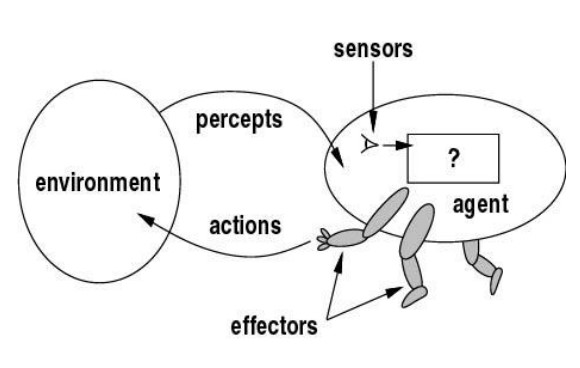
\includegraphics[width=0.7\textwidth]{immagini/Agenti_intelligenti.jpg}
	\caption*{Agente intelligente}
\end{figure}

\subsubsection{La sfida: RoboCup}
La \textit{Robot World Cup Initiative} (RoboCup) è un problema di riferimento per la ricerca in I.A.\
Si tratta di realizzare agenti in grado di giocare a calcio (entro il 2050!).\
Un problema difficile, da usare come banco di prova per nuove idee e tecnologie.

Tecnologie da sviluppare e integrare

\begin{itemize}
	\item agenti autonomi
	\item collaborazione tra agenti
	\item acquisizione di strategie
	\item ragionamento e pianificazione in tempo reale
	\item robotica
	\item tecnologie hw e sw per infrastruttura
\end{itemize}

\subsubsection{Capacità di emozioni?}

\begin{center}
	``\textit{The question is not whether intelligent machines can have emotions, but whether machines can be intelligent without any emotions}.''

	[Minsky, The Society of Mind]

\end{center}
Capacità di comprendere e mostrare emozioni $\rightarrow$ ruolo delle emozioni nel meccanismo di decisione.

\section{The AI revolution?}

\begin{itemize}
	\item Algoritmi di apprendimento automatico che estraggono modelli statistici predittivi da immense quantità di esempi.
	\item Tecniche di estrazione di ``\textit{significati}'' da grande quantità di testi.
	\item Sistemi in grado di rispondere a domande in linguaggio naturale in un ``dominio aperto''.
\end{itemize}

\subsubsection{La disponibilità di grosse quantità di dati}
L'enfasi si sposta dagli algoritmi ai dati e agli algoritmi di apprendimento (ML e DM).\
Esempi dalle tecnologie del linguaggio:
\begin{itemize}
	\item La traduzione automatica di Google
	\item L'interazione in linguaggio naturale di SIRI
\end{itemize}
Più dati, maggiore l'accuratezza,\ \dots\ apparentemente senza limite (``Unreasonable Effectiveness of Big Data'')

La domanda diventa:\ l'intelligenza può essere estratta o inferita dai dati?

\subsubsection{The \textit{deep learning} tsunami}

L'idea di usare reti neurali con molti livelli (deep NN) era stata tentata per diversi anni, ma solo verso il 2011 si riescono ad avere successi evidenti, come riconoscimento di immagini e parlato.

C. Manning:\ ``le reti neurali profonde sono in giro da un po' di anni ma nel 2015 hanno colpito come uno tsunami il settore del NLP''.

I maggiori esperti (Le Cun, Hinton, Benjo) sono concordi nel ritenere che ci saranno sviluppi importanti a breve nella comprensione dei testi, video, traduzione automatica, QA,\ \dots

Apprendimento di Deep Networks diviene praticabile dal punto di vista computazionale:
\begin{itemize}
	\item Possibilità di usare GPU multiple (Graphic Processing Unit); ottimizzate per il prodotto di matrici.
	\item Se avessimo usato gli stessi algoritmi 10 anni fa, non avrebbero ancora finito.
\end{itemize}

\subsection{Priorità di ricerca}
L'intelligenza artificiale\dots ``deve fare solo quello che noi vogliamo che faccia''.\
Servono ricerche non solo per rendere l'IA più \textbf{capace} ma anche fare in modo che sia \textbf{robusta} e \textbf{benefica} per la società (\textit{Trustworthy AI})
\begin{itemize}
	\item Impatto economico sul mercato del lavoro e sulla società
	\item Responsabilità dei veicoli autonomi, etica delle macchine, armi autonome, privacy
	\item Verifica (il sistema è ``corretto''?), validità (il sistema è ``giusto''?)
	\item Sicurezza (protezione da terzi), controllo (dei sistemi autonomi)
\end{itemize}

\section{In sintesi}
È difficile dare una definizione univoca di ``intelligenza'' e quindi di ``intelligenza artificiale''.\
A seconda dei periodi storici gli approcci sono diversi, l'enfasi è diversa, gli obiettivi stessi sono diversi.\
Parafrasando la definizione di Kurzweil

\begin{center}
	\textit{A.I è l'arte di creare macchine che svolgono funzioni che tuttora richiedono intelligenza umana per essere svolte}

	\dots \textit{un ``bersaglio mobile''}.
\end{center}
A.I. (ML) come alternativa all'approccio algoritmico tradizionale in presenza di incertezza.
\begin{itemize}
	\item \textit{Sorgenti di incertezza:\ sensori imperfetti, dati incompleti, limiti alle capacità di calcolo}
	\item \dots
	\item \textit{Thrun:\ AI is the technique of uncertainty management in computer software.\ AI is the discipline that you apply when you don't know what to do.}
\end{itemize}
Ma ricordate:\ l'IA non coincide con il ML;\ la General AI è ancora lontana e dovrà integrare diverse capacità e in particolare apprendimento e ragionamento.
